\documentclass{article}
\usepackage[utf8]{inputenc}
\usepackage{algorithm}
\usepackage{algpseudocode}
\usepackage{float}
\usepackage{amsmath}
\usepackage{graphicx}
\usepackage{hyperref}
\hypersetup{
    colorlinks=true,
    linkcolor=blue,
    filecolor=magenta,      
    urlcolor=cyan,
    pdftitle={Overleaf Example},
    pdfpagemode=FullScreen,
    }
\title{Homework No.3}
\author{Ruqi Feng}
\date{September 2022}

\begin{document}

\maketitle

\section{Time Complexity of Gaussian Elimination}
\subsection{Problem Description}
Prove that the time complexity of the Gaussian elimination algorithm is $O(N3)$.
\subsection{Proof}
Suppose the linear equations to solve is
\begin{equation}
    Ax = b
\end{equation}
and matrix $A$ is an $n$ by $n$ matrix and has full-rank.
Then Gaussian elimination involves 2 major steps:
\paragraph{a. Transform into Row Echelon Form}
Perform row operations to make entries in the coefficient matrix below the diagonal zero. In the $i$-th column, there are $n-i$ entries that needs to be set zero, which requires $n - i$ row operations. In each row operation, roughly $n - i$ multiplications and $n - i$ additions are required. Therefore, the total operation number needed is approximately
\begin{equation}
    N\approx\sum_{i=1}^{n-1} 2(n-i)(n - i) \approx \frac{2n^3}{3}
\end{equation}
Therefore, this step requires time complexity of $O(n^3)$
\paragraph{b. Back substitution}
After reducing the coefficient matrix into REF, the solution can be found easily.
From bottom to top, find $x_n$ and insert into $A_{n-1}x_{n-1} + A_{n}x_n=b_{n-1}$ and so on. When solving the $i$-th linear equation, about $3i$ operations are need, so the time complexity of this step is $O(n^2)$
\par\quad\par
Using the addition rule of time complexity, the time complexity of Gaussian elimination is 
\begin{equation}
    O(n^3)+O(n^2)=O(n^3)    
\end{equation}



\section{Transformation into RREF}

\subsection{Problem Description}
Write a general code to transform a n*m matrix into the REDUCED ROW ECHELON FORM, and use the code to obtain the RREF of the following matrix. [2, 8, 4, 2; 2, 5, 1, 5; 4, 10, -1, 1]

\subsection{My Approach}
The procedure to find RREF is similar to Gaussian elimination. There are two majors steps which I call 'forward elimination' and 'backward elimination'.\par
In 'forward elimination', entries below the diagonal will be set to zero and the diagonal entries will be set to 1. Before setting the $j$-th column, the $j$-th row ($j\le n$) is rescaled so that the diagonal entry in it is set to $1$. 
If the $j$-th diagonal entry is zero or too small, appropriate entries ($a_{xj}$ where $x>j$) in rows below will be found and those rows are swapped with the $j$-th row. 
\par
However, if a certain row does not have a valid pivot and every entry below it is invalid as well, the RREF does not exist in this case. This is because the entries the diagonal entry in this row will not be able to be eliminated in the backward elimination. My program will print an error message when calling the print function of the returned instance in this case.
\par
Then the entry $a_{ij}$ (suppose $j<i$) is set to zero by multiplying the $j$-th row by $-a_{ij}$ and add it to the $i$-th rows.
After forward elimination, the matrix will become\par
\begin{equation}
    \begin{pmatrix}
        1 & a_{12} & a_{13} & b_1 \\
        0 & 1 & a_{23} & b_2 \\
        0 & 0 & 1 & b_3 \\
    \end{pmatrix}
\end{equation}
or with rows of all zero entries in the lowest rows
\begin{equation}
\label{eq:RREF_example_2}
    \begin{pmatrix}
    1 & a_{12} & a_{13} & b_1 \\
    0 & 1 & a_{23} & b_2 \\
    0 & 0 & 1 & b_3 \\
    0 & 0 & 0 & 0\\
    0 & 0 & 0 & 0
    \end{pmatrix}
    \mbox{or}
    \begin{pmatrix}
    1 & a_{12} & a_{13} & b_1 \\
    0 & 1 & a_{23} & b_2 \\
    0 & 0 & 1 & b_3 \\
    0 & 0 & 0 & 1\\
    0 & 0 & 0 & 0
    \end{pmatrix}
\end{equation}
in which cases, the program will execute the backward elimination procedure. Although in the matrix on the right in Eq.\ref{eq:RREF_example_2} the system of linear equations corresponding to the matrix has no solutions, the RREF of it still exists.
\par
If the RREF exists, the program will continue to execute 'backward elimination', where the elements above pivots are set to zero by adding the $j$-th row, multiplied by $-a_{ij}$, to the $i$-th row. The result is RREF of the input matrix, then.

\subsection{Pseudocode}
\begin{algorithm}[H]% the algorithm block floats in the page 
\caption{RREF of a given matrix}
    \begin{algorithmic}[1]% This number indicates the line number to start labeling with line number.
        \Statex\textbf{Input:} an input matrix, $A$
        \Statex\textbf{Output:} RREF of the input matrix
        \State $n\gets$ row number of $A$
        \For{$i\gets 1$ to $n$}
            \If{$|a_{ii}| < 10^{-10}$}
                \State swap the $i$-th row with argmax($A[i, i+1:]$)-th row
                \If{$|a_{ii} < 10^{-10}|$}
                    \Return 'RREF does not exist'
                \EndIf
            \EndIf
            \For {$j\gets i+1$ to $n$}
                \For{$k\gets i$ to $n$}
                    \State $a_{jk}\gets a_{jk}-a_{ji}a_{ik}$
                \EndFor
            \EndFor
        \EndFor
        \For {$i\gets 1$ to $n$}
            \For {$j\gets 1$ to $i-1$}
                \For {$k\gets i$ to $n$}
                  \State $a_{jk}\gets a_{jk}-a_{ji}a_{ik}$
                \EndFor
            \EndFor
        \EndFor
    \end{algorithmic}
\end{algorithm}

\subsection{Input and Outputs}

The matrix required in the problem description is solved. The output is 
\begin{equation}
\begin{pmatrix}
1.0& 0.0& 0.0& 11.0\\
0.0& 1.0& 0.0& -4.0\\
-0.0& -0.0& 1.0& 3.0
\end{pmatrix}
\end{equation}
as is shown in test case 1.
\par
Test case 2 and 3 are cases where the row of the input matrix is more than the columns. In test case 6 the entries are chosen so that the second column has no valid pivot. My program works fine in these test cases, shown in Fig.\ref{fig:Q2screenshot}\par
The source code file Q2\_RREF.py can be run in the terminal and no external packages are required.

\begin{figure}[ht]
    \centering
    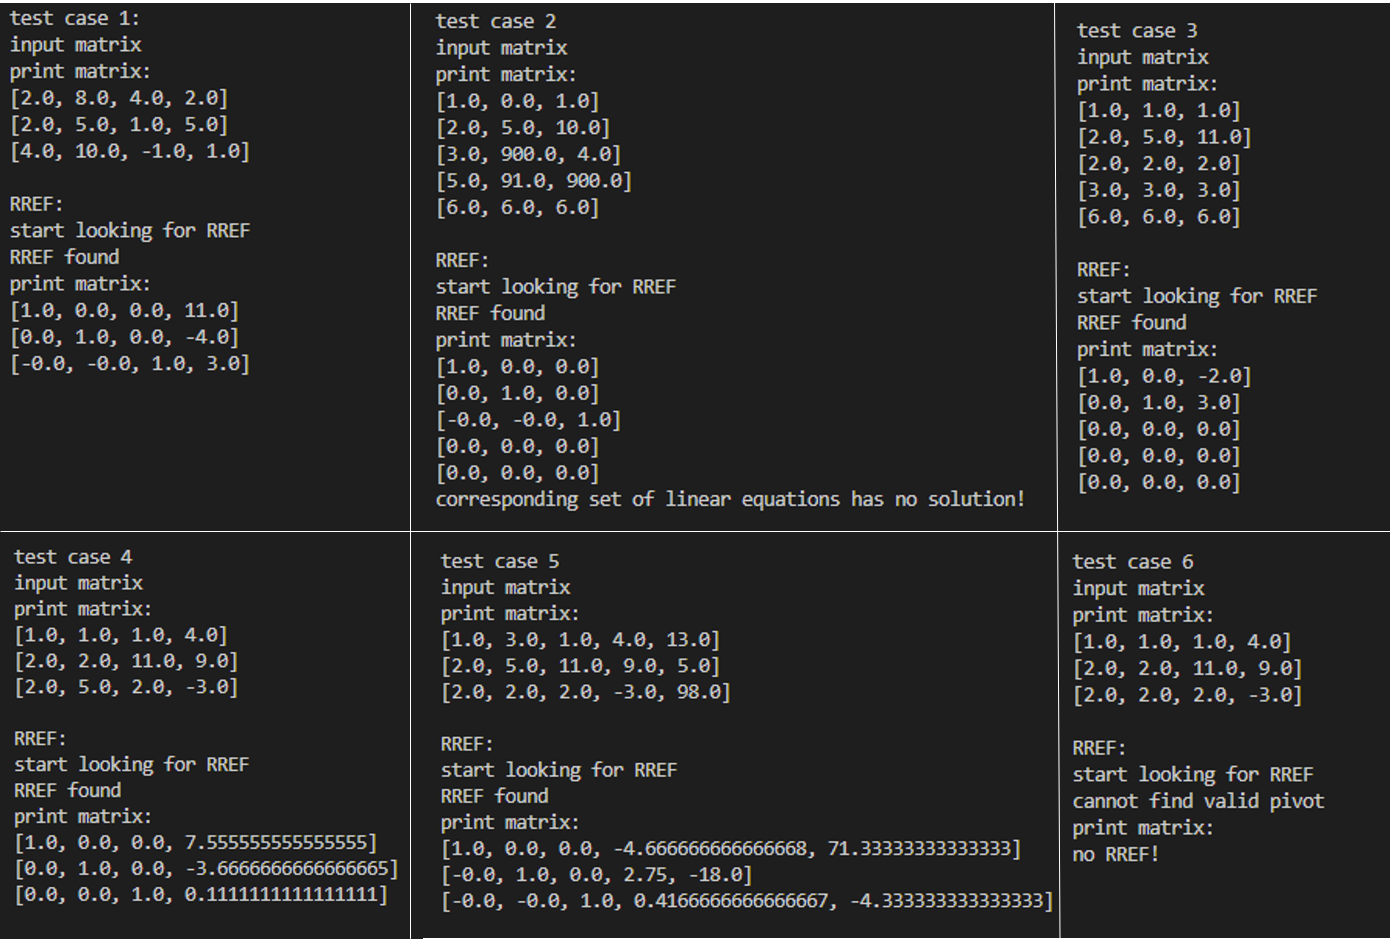
\includegraphics[width=1\textwidth]{Q2screenshot.png}
    \caption{Screenshot of test cases in Q2}
    \label{fig:Q2screenshot}
\end{figure}
\newpage

\section{Solve Schrodinger Equations}

\subsection{Description}

Solve the 1D Schrodinger equation with the potential (i) V(x)= $x^2$; (ii) V(x)= $x^4-x^2$ with the variational approach using a Gaussian basis (either fixed widths or fixed centers). Consider the three lowest energy eigenstates. 

\subsection{Analysis and solution}

Searching for a certain state is equivalent to searching for the linear combination of a set of (somewhat appropriate, if not complete) basis. Suppose the basis are $\phi_i$ and some state can be linearly represented by the basis $\psi = \sum_i c_i \phi_i$. We then want the expectation of the energy of the state $\psi$ to be minimized, that is, 
\begin{align}
    \frac{\partial \langle H\rangle}{\partial c_i} = \partial_{c_i}\frac{\sum_{ij}\langle c_i\phi_i|H c_j\phi_j\rangle}{\sum_{ij}\langle c_i\phi_i|\phi_j c_j\rangle}
\end{align}
denoting $\langle \phi_i H\phi_j \rangle$ as $H_{ij}$ and $\langle \phi_i \phi_j \rangle$ as $S_{ij}$ (the basis we chose are not necessarily orthonormal). 
\begin{align}
    \sum_jc_jH_{ij}&=\frac{\sum_{ij}c_ic_jH_{ij}}{\sum_{ij}c_ic_jS_{ij}}\sum_jc_jS_{ij}\\
    H\vec{c} &= E S\vec{c}\label{generalized_eigenvalue_problem}
\end{align}
where $E$ is $\frac{\sum_{ij}c_ic_jH_{ij}}{\sum_{ij}c_ic_jS_{ij}}$ which is, by definition, the expectation value of Hamiltonian. Meanwhile, Eq.\ref{generalized_eigenvalue_problem} is a generalized eigenvalue problem, where $E$ is the eigenvalue. The problem can be solved by taking the square root of $S$ and converting Eq.\ref{generalized_eigenvalue_problem} into
\begin{equation}
    H'\vec{c'} = E\vec{c'}
\end{equation}
where $H'=S^{-\frac{1}{2}}HS^{-\frac{1}{2}}$, and $\vec{c'}=S^{\frac{1}{2}}\vec{c}$.\par

In our numerical solution, the matrix calculations are relatively straightforward with the help of all sorts of available linear algebra packages, such as numpy and scipy. What we are left to do is to select a set of proper basis and then calculate $H_{ij}$ and $S_{ij}$. Integrations are done numerically in my program. As for basis choices, the eigenstates in the harmonic potential Hamiltonian are Gaussian functions, so we choose them as our basis. To construct a set of basis, we need to vary some parameters in the wavefunction. Suppose a Gaussian function is expressed as
\begin{equation}
    \phi = (\frac{2\nu}{\pi})^{1/4} e^{-\nu(x-s)^2}
\end{equation}
where $m$, $\hbar$ has been set to $1$ and $\omega$ set to $\sqrt{2}$ (this will keep the harmonic potential in the form of $x^2$). By choosing a series of $\nu$ or a series of $s$, we are able to produce different basis, as shown in Fig.\ref{fig:dif_center} and Fig.\ref{fig:dif_width}.

\begin{figure}[!htb]
    \centering
    \begin{minipage}{0.5\textwidth}
        \centering
        \includegraphics[width=1\linewidth]{dif_width_5.png}
        \caption{basis with different width}
        \label{fig:dif_width}
    \end{minipage}%
    \begin{minipage}{0.5\textwidth}
        \centering
        \includegraphics[width=1\linewidth]{basis.png}
        \caption{basis with different center position}
        \label{fig:dif_center}
    \end{minipage}
\end{figure}

It is also of importance how many basis to choose and how dense their intervals are. If there are not enough number of basis, the result may be inaccurate, as shown in Fig.\ref{fig:V2_center_25_basis} (the basis have different center location varying in $[-10, 10]$). However, when the number is increased from $25$ to $35$, the calculated eigenfunctions are more accurate. On the other hand, there can not be too many basis, otherwise the inner product with each other will be close to the inner product with itself. This will result in larger non-diagonal entries in matrix $S$, and thus potentially produce imaginary eigenvalues of $H$, which is unphysical. (Though $H$ itself is a symmetrical matrix, we are solving a generalized eigenvalue problem and $H'$ is not necessarily symmetrical) Adding basis in a wider range seems to help but basis 'outside' the range of the potential well can only introduce slight improvement to the solution. It seems that a trade-off is inevitable.

\begin{figure}[!htb]
    \centering
    \includegraphics[width=1\textwidth]{V2_dif_center_basisnum=25.png}
    \caption{25 basis, result is not ideal}
    \label{fig:V2_center_25_basis}
\end{figure}
\begin{figure}[!htb]
    \centering
    \includegraphics[width=1\textwidth]{V2_dif_center_basisnum=35.png}
    \caption{35 basis, result is more accurate}
    \label{fig:V2_center_35_basis}
\end{figure}

Luckily, after some trials, I've found that in most cases enough basis are allowed to produce an accurate enough result before failing due to non-positive-definite $S$ matrix. In the following sections, $\nu$ will be varied in $[0.1, 1]$ with $s=0$ while $s$ will be varied in $[-10, 10]$ with $\nu=3$. Furthermore, I've found better choices of the basis can give precise results with fewer number of basis, which will be included in Sec.\ref{sec:discussion}.


\subsection{Pseudocode}
\begin{algorithm}[H]% the algorithm block floats in the page 
\caption{RREF of a given matrix}
    \begin{algorithmic}[1]% This number indicates the line number to start labeling with line number.
        \Statex\textbf{Input:} $n$ basis {$\phi_i$} and potential $V(x)$
        \Statex\textbf{Output:} eigenvalues $E$ and eigenstates$\psi$ of the Hamiltonian
        \For{$i$ in range($n$)}
            \For {$j$ in range($n$)}
                \State $H_{ij}\gets\int\phi_i(\partial_x^2 + V(x))\phi_jdx$
                \State $S_{ij}\gets\int\phi_i\phi_jdx$
            \EndFor
        \EndFor
        \State $D, U\gets$ eigenvalues and matrix of eigenvectors of $S$
        \State $S^{\frac{1}{2}}\gets UD^{\frac{1}{2}}$
        \State $S^{-\frac{1}{2}}\gets $ inverse of $S^{\frac{1}{2}}$
        \State $H'\gets S^{-\frac{1}{2}} HS^{-\frac{1}{2}}$
        \State $E, C'\gets$ eigenvalues and matrix of eigenvectors of $H'$
        \State $C\gets S^{-\frac{1}{2}} C'$
        \State $\psi_i\gets\sum_{j=1}^n C_{ij}\phi_j$
        \State Sort $E$ and $\psi_i$ according to $E$
    \end{algorithmic}
\end{algorithm}

\subsection{Results}
\subsubsection{How to run the program}
The file Q3\_schrodinger.py can be run from the terminal. Python packages numpy, matplotlib and tqdm are required.
\subsubsection{Lowest 3 states}
\textbf{Solve for $V_1$}\par
The first potential is $V(x) = x^2$, which is the harmonic oscillator potential. As mentioned above, the parameters are chosen so that the potential has the form $\frac{m\omega^2x^2}{2}$. The theoretically correct eigenvalues of Hamiltonian are $(0.5+n)\hbar\omega$, where $\hbar=1$ and $\omega=\sqrt{2}$, respectively. As shown in table\ref{table:V1}.\par
It can be noticed that simply varying $\nu$ in Gaussian wave packets cannot produce the first activated state because the basis are even while those states are odd. No matter how many basis are added, as long as they are even, odd eigenstates are `skipped', as shown in Fig.\ref{fig:V1_even_only}. On the other hand, by varying the center, odd functions can be created. In order to overcome this problem, I add a set of odd basis to the even set, namely
\begin{equation}\label{basis_odd_and_even}
    \phi_i = x(\frac{2\nu}{\pi})^{1/4} e^{-\nu(x-s)^2}
\end{equation}
It does not matter that the basis are not normalized, because the produced eigenstates will be normalized once more. The resulting eigenvalues are also listed in \ref{table:V1} and the wave functions are plotted in Fig.\ref{fig:V1_even_and_odd}\par

\begin{figure}[!htb]
    \centering
    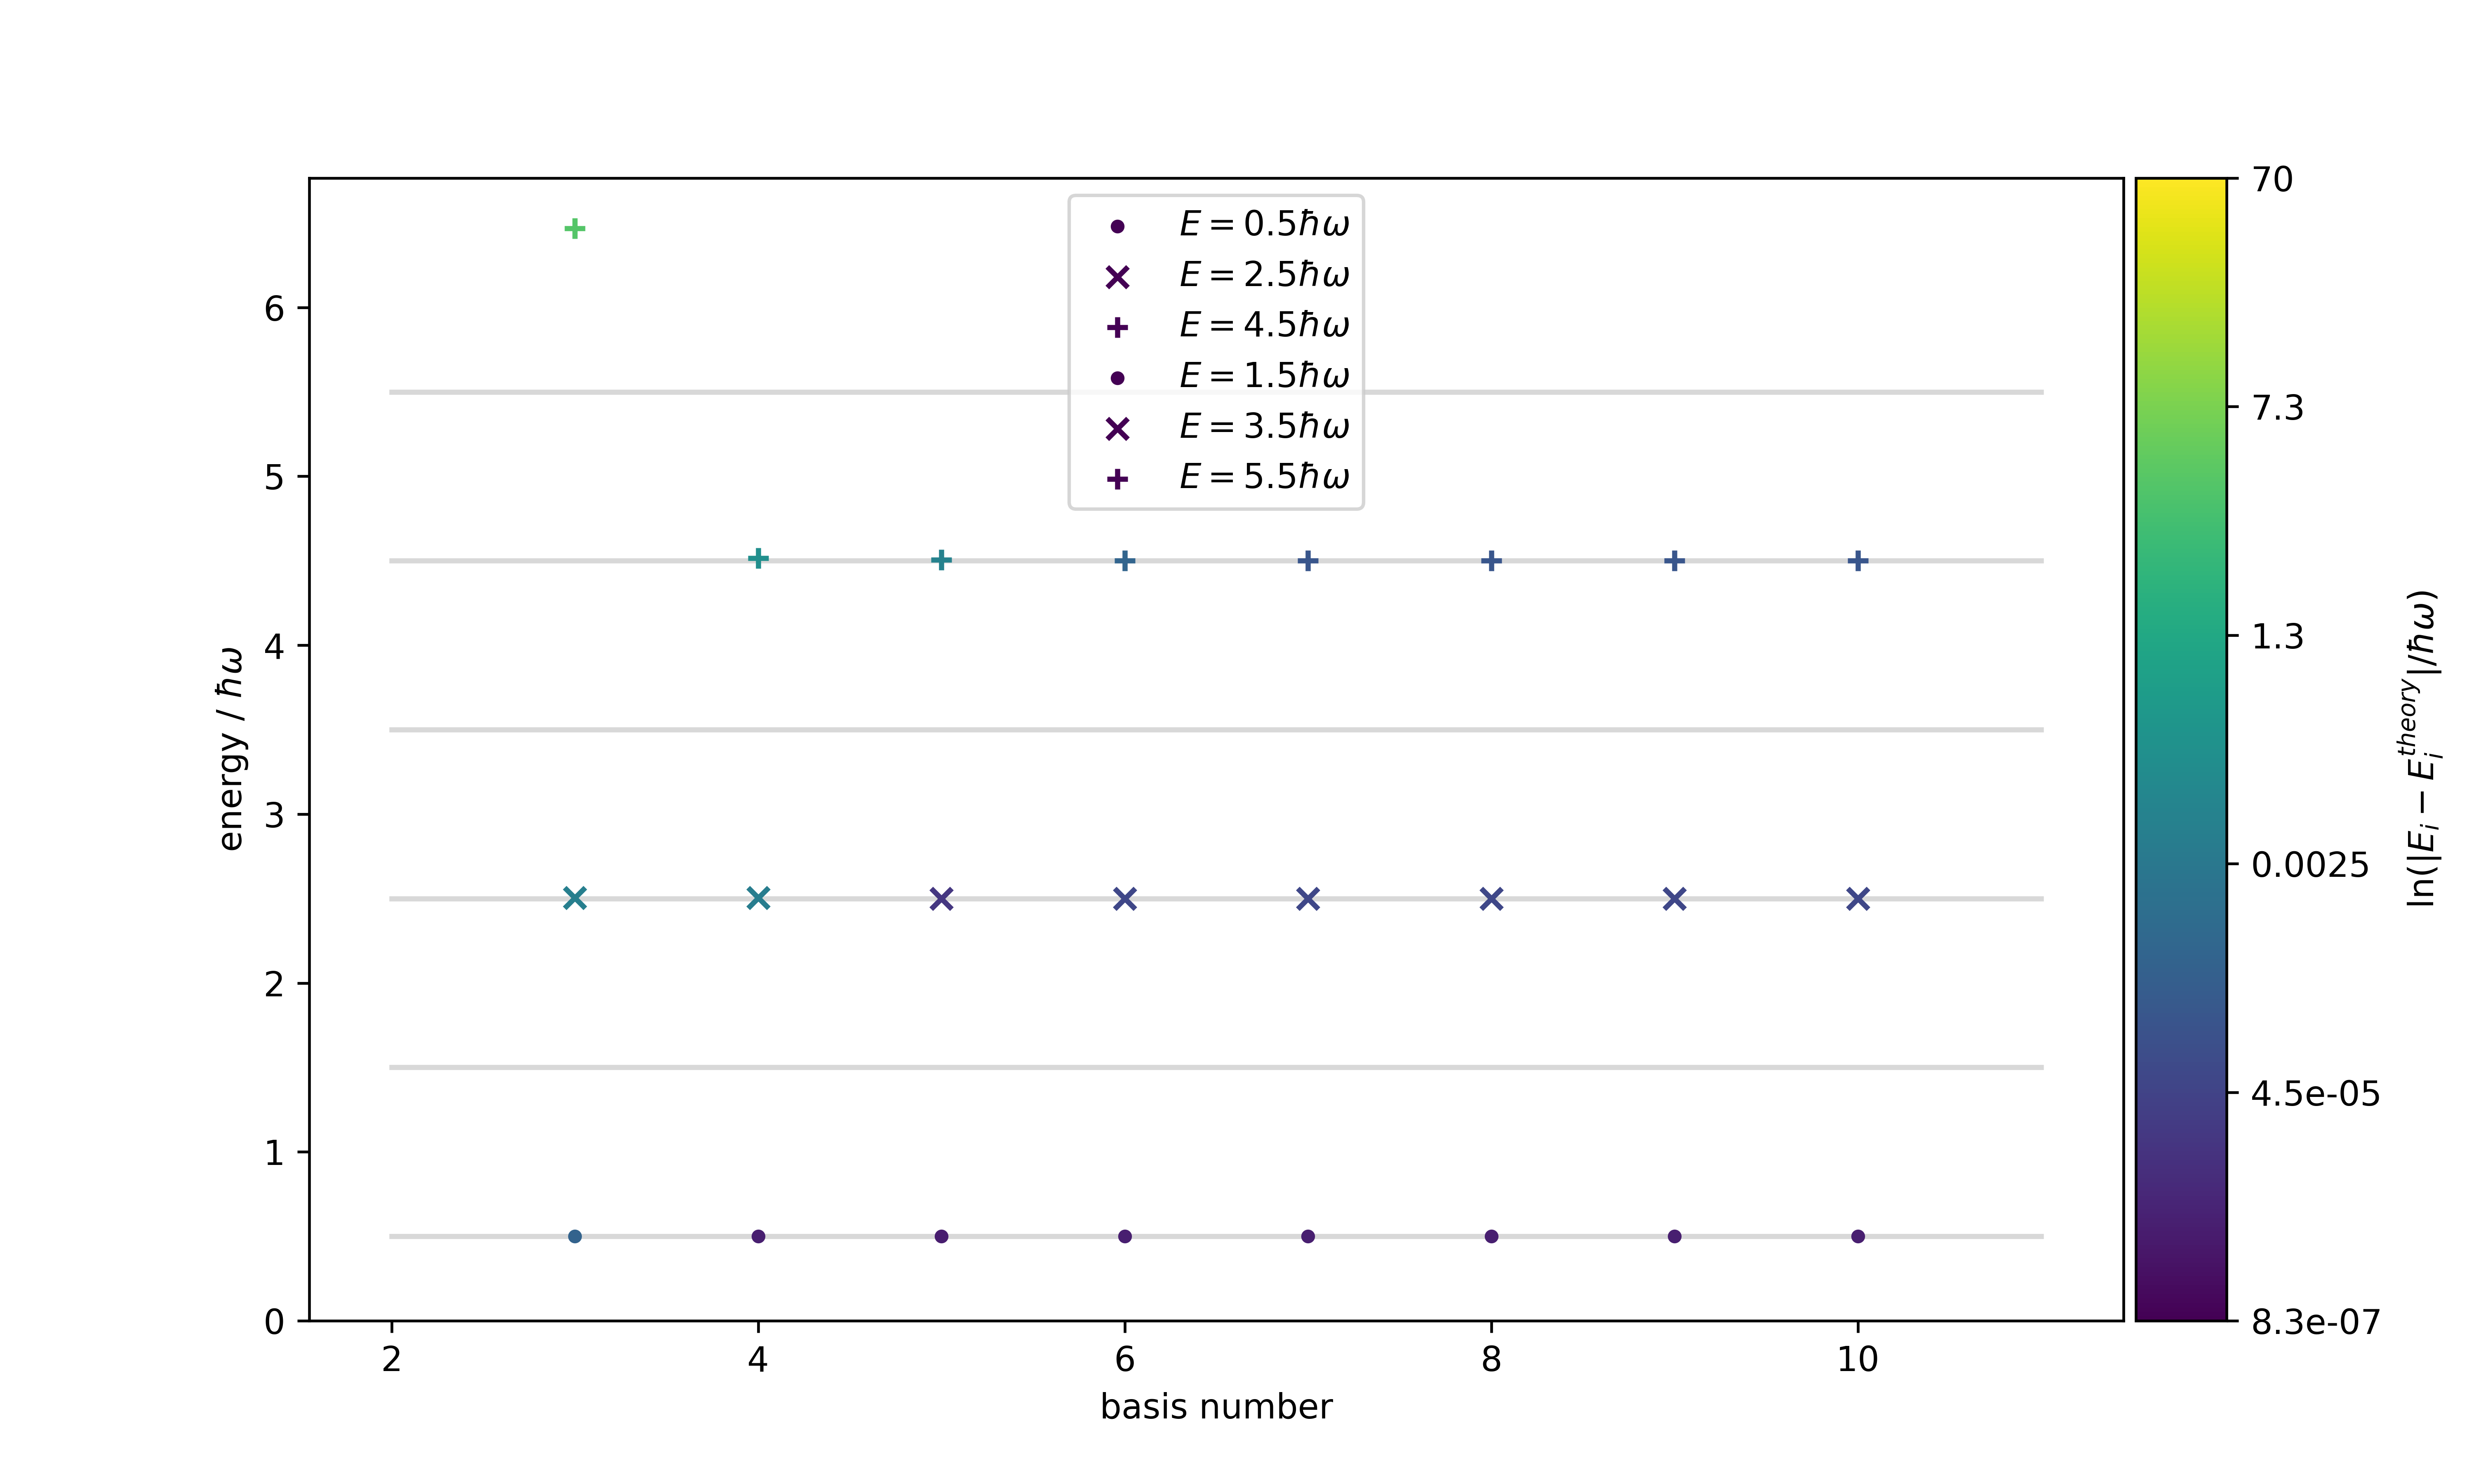
\includegraphics[width=1\textwidth]{V1_even_dif_basis_num.png}
    \caption{Basis are created by varying width of Gaussian functions. Only even eigenstates of the Hamiltonian are produced, with energy $(2n+\frac{1}{2})\hbar\omega$. The grey lines are theoretical energies and the energies of odd states are `skipped'.}
    \label{fig:V1_even_only}
\end{figure}

\begin{center}
    \begin{tabular}{c|c|c|c|c}
        \hline
         &basis num& $E_0/\hbar\omega$ & $E_1\hbar\omega$ & $E_2\hbar\omega$\\
        \hline        
        vary centers $s$ &40& 0.50000 &1.499998 & 2.49996\\
        vary widths $\nu$ & 10 &0.50000& &2.49994\\
        vary widths $\nu$ (even and odd)& 20 & 0.50000 & 1.499997& 2.49999\\
\hline
    \end{tabular}\label{table:V1}
\end{center}

\begin{figure}[!htb]
    \centering
    \includegraphics[width=1\textwidth]{wavefuncplot_basis_num=10.png}
    \caption{Eigenfunctions of $V_1$. The blue ones are odd states while the orange ones are even.}
    \label{fig:V1_even_and_odd}
\end{figure}
\textbf{Solve for $V_2$}\par
The second potential is $V(x)=-x^2+x^4$, or $(-(\frac{x}{x_0})^2 + (\frac{x}{x_0})^4)\frac{m\omega^2x_0^2}{2}$ where $x_0=1$, $\hbar=1$ and $\omega=\sqrt{2}$, to be exact. To find the odd states, we substituted the varying width $\nu$ of Gaussian basis with varying width $\nu$ of both Gaussian and basis in Eq.\ref{basis_odd_and_even}. The varying center $s$ basis are also used and compared with the previous basis. The calculated 3 lowest eigenvalues are shown in Fig.\ref{table:V2}, and it can be identified that the two choices of basis give very close results. As is shown in Fig.\ref{fig:V2_centers} and Fig.\ref{fig:V2_even_and_odd} (they are in theory identical except for an overall phase difference), the wave functions are 'fatter' compared to those in $V_1$ because the buttom of potential $V_2$ is wider.

\begin{center}
    \begin{tabular}{c|c|c|c|c}
        \hline
         &basis num& $E_0/\hbar\omega$ & $E_1\hbar\omega$ & $E_2\hbar\omega$\\
        \hline        
        vary centers $s$ &70& 0.238970 &1.140342 & 2.589210\\
        vary widths $\nu$ (even and odd)& 20 & 0.238984 & 1.140456& 2.589428\\
        \hline
    \end{tabular}\label{table:V2}
\end{center}
\begin{figure}[!htb]
    \centering
    \includegraphics[width=1\textwidth]{V2_width_odd_and_even_wavefuncplot_basis_num=10.png}
    \caption{Eigenstates of $V_2$ produced with basis in Eq.\ref{basis_odd_and_even} and Gaussian functions with varying width}
    \label{fig:V2_even_and_odd}
\end{figure}
\begin{figure}[!htb]
    \centering
    \includegraphics[width=1\textwidth]{V2_center_wavefuncplot_basis_num=70.png}
    \caption{Eigenstates of $V_2$ produced by Gaussian functions with varying center}
    \label{fig:V2_centers}
\end{figure}

\subsubsection{Discussions}
\label{sec:discussion}
As you may have noticed, when choosing the 'varying center Gaussian' basis, the required basis number is larger than 'varying width Gaussian and Eq.\ref{basis_odd_and_even}' basis. By changing the number of basis and examining the difference between the calculated eigenvalues and theoretical values, the difference between the two types of basis can be shown clearly when comparing Fig.\ref{fig:V1_dif_basis_num_center}
and Fig.\ref{fig:V1_dif_basis_num_even_and_odd}. I think the reason is that in a symmetrical potential like $V_1$ and $V_2$, Gaussian functions or Eq.\ref{basis_odd_and_even} centered at $x=0$ are closer to actual eigenfunctions. The difference in required number of basis is even more drastic when it comes to $V_2$, where the 'varying center Gaussian' basis gives eigenvalues hundreds of times of the actual value with few basis numbers while 'varying width Gaussian and Eq.\ref{basis_odd_and_even}' basis are already able to give relatively good results. These are shown in Fig.\ref{fig:V2_dif_basis_num_even_and_odd} and Fig.\ref{fig:V2_dif_basis_num_center}.
\begin{figure}[!htb]
    \centering
    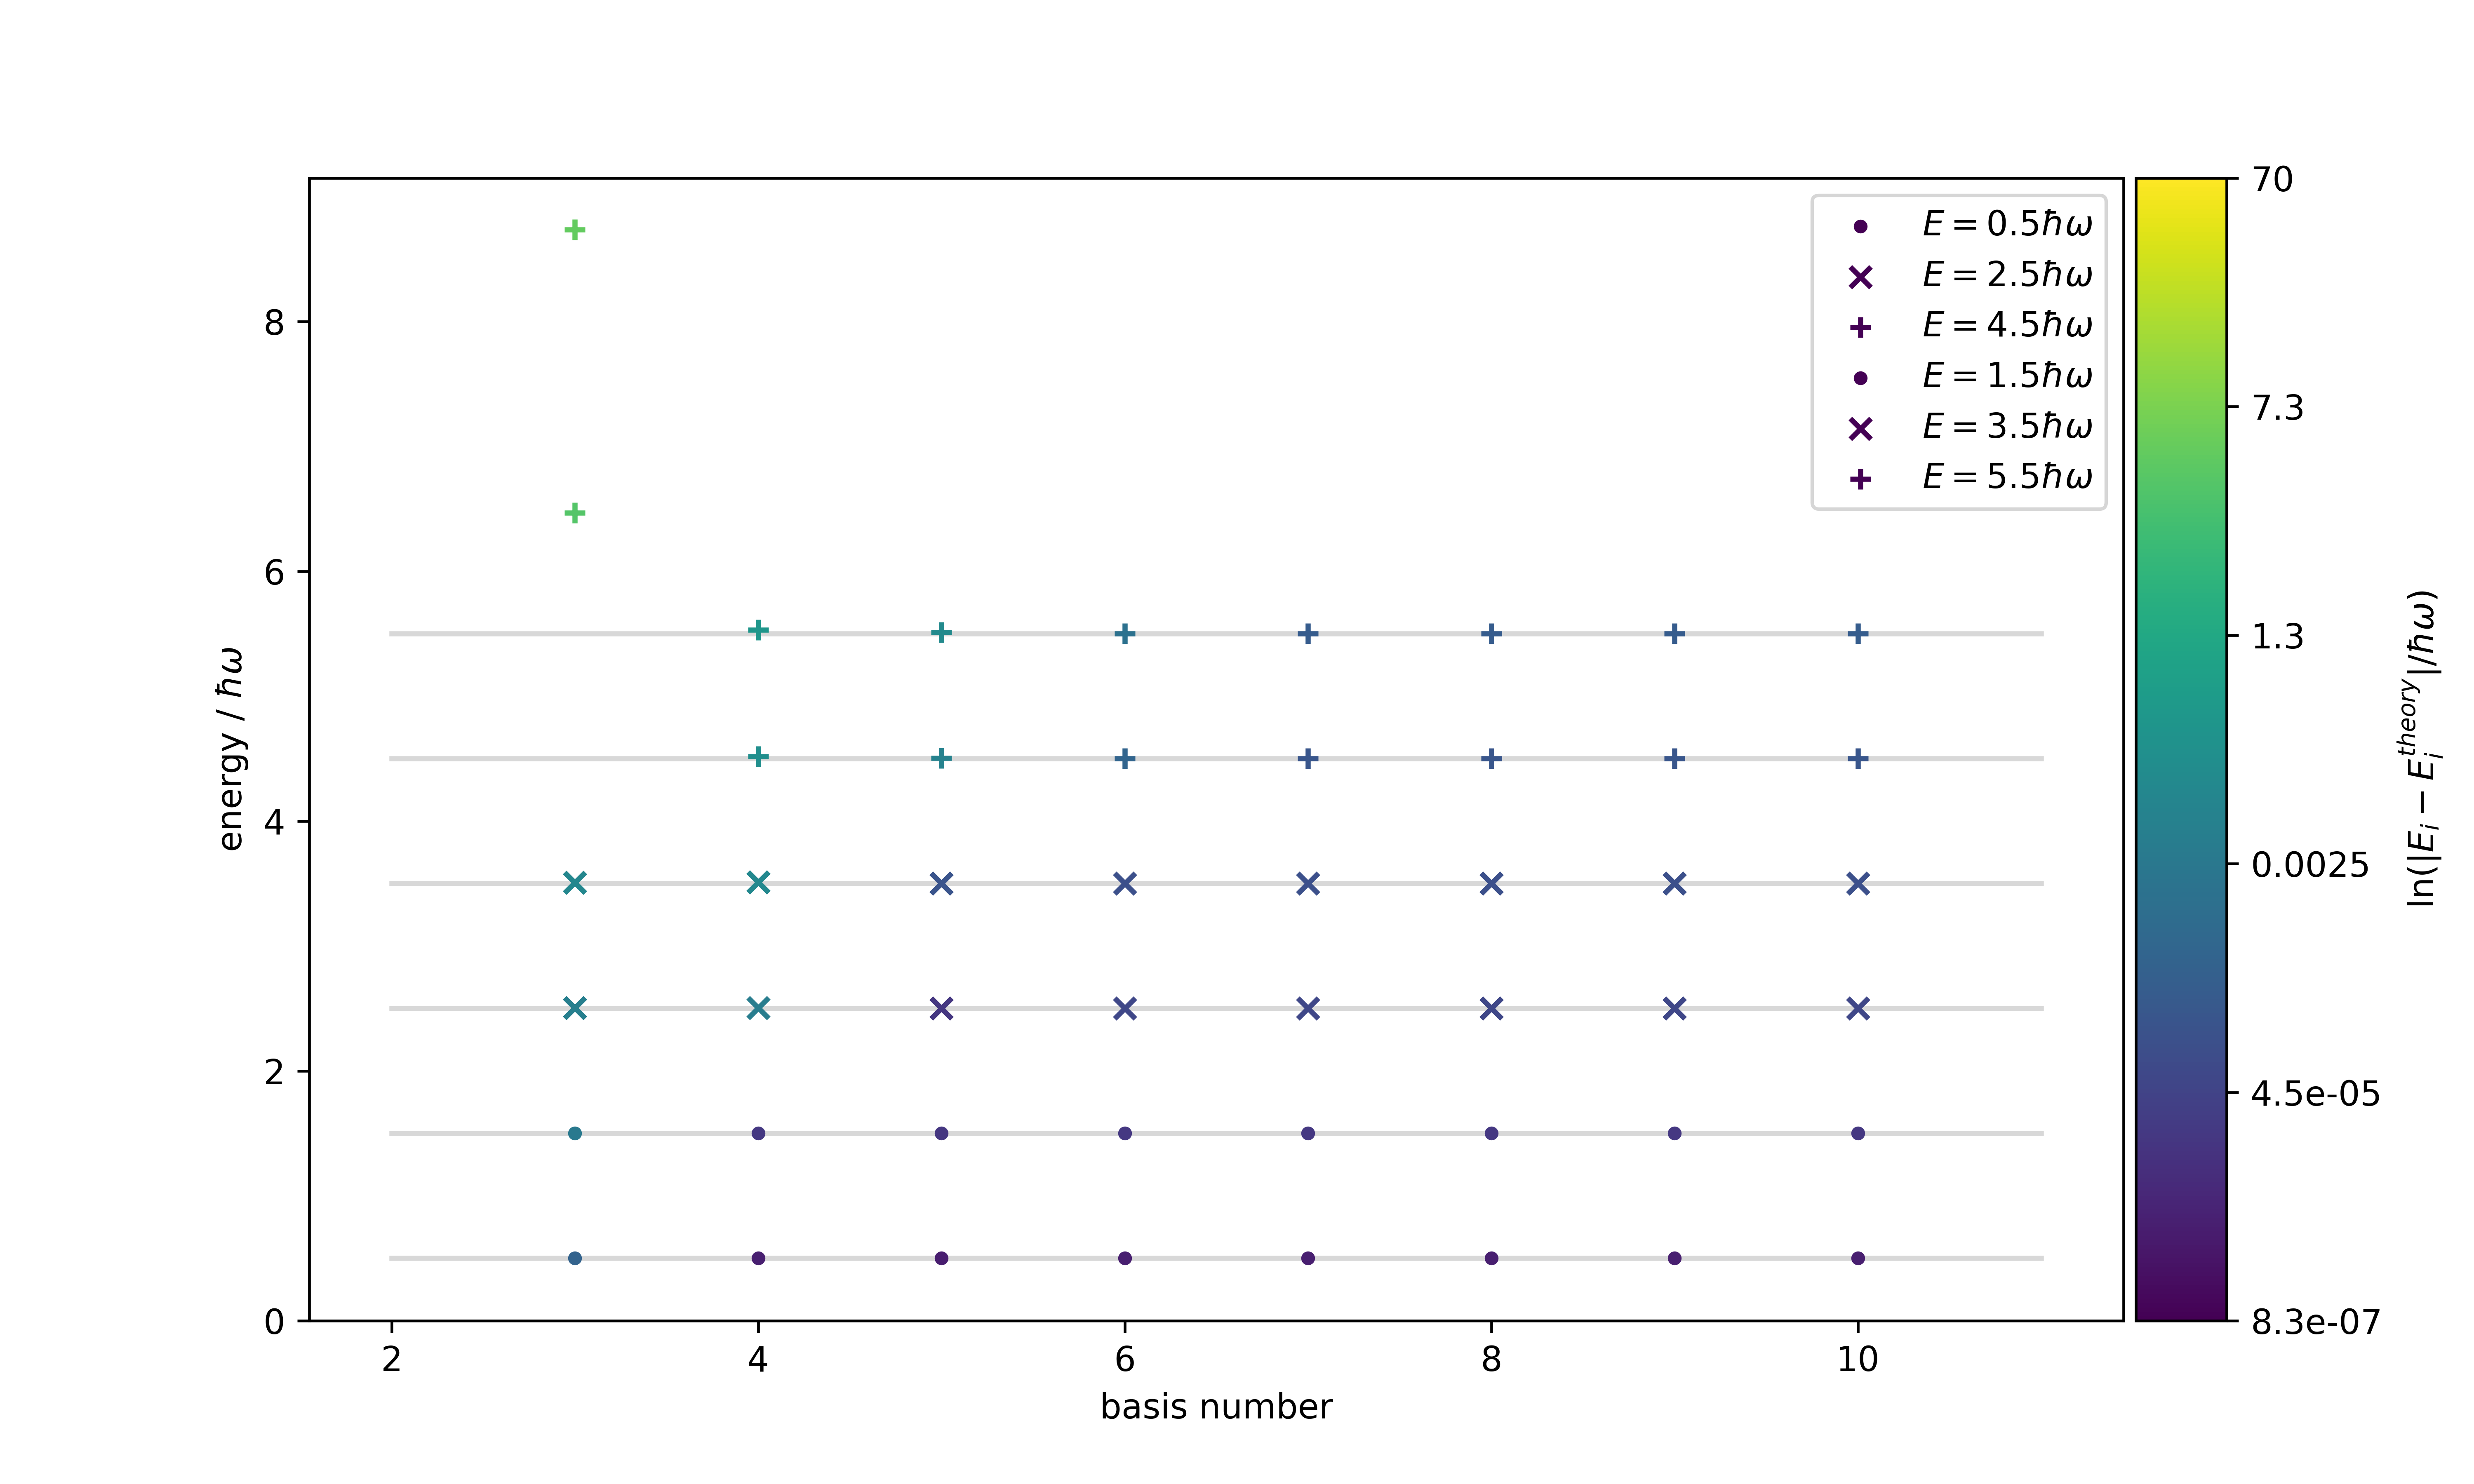
\includegraphics[width=1\textwidth]{V_1_enven_and_odd-different basis number.png}
    \caption{Few basis can produce accurate results. The color characterizes how close the numerical result is to the theoretical value.}
    \label{fig:V1_dif_basis_num_even_and_odd}
\end{figure}

\begin{figure}[!htb]
    \centering
    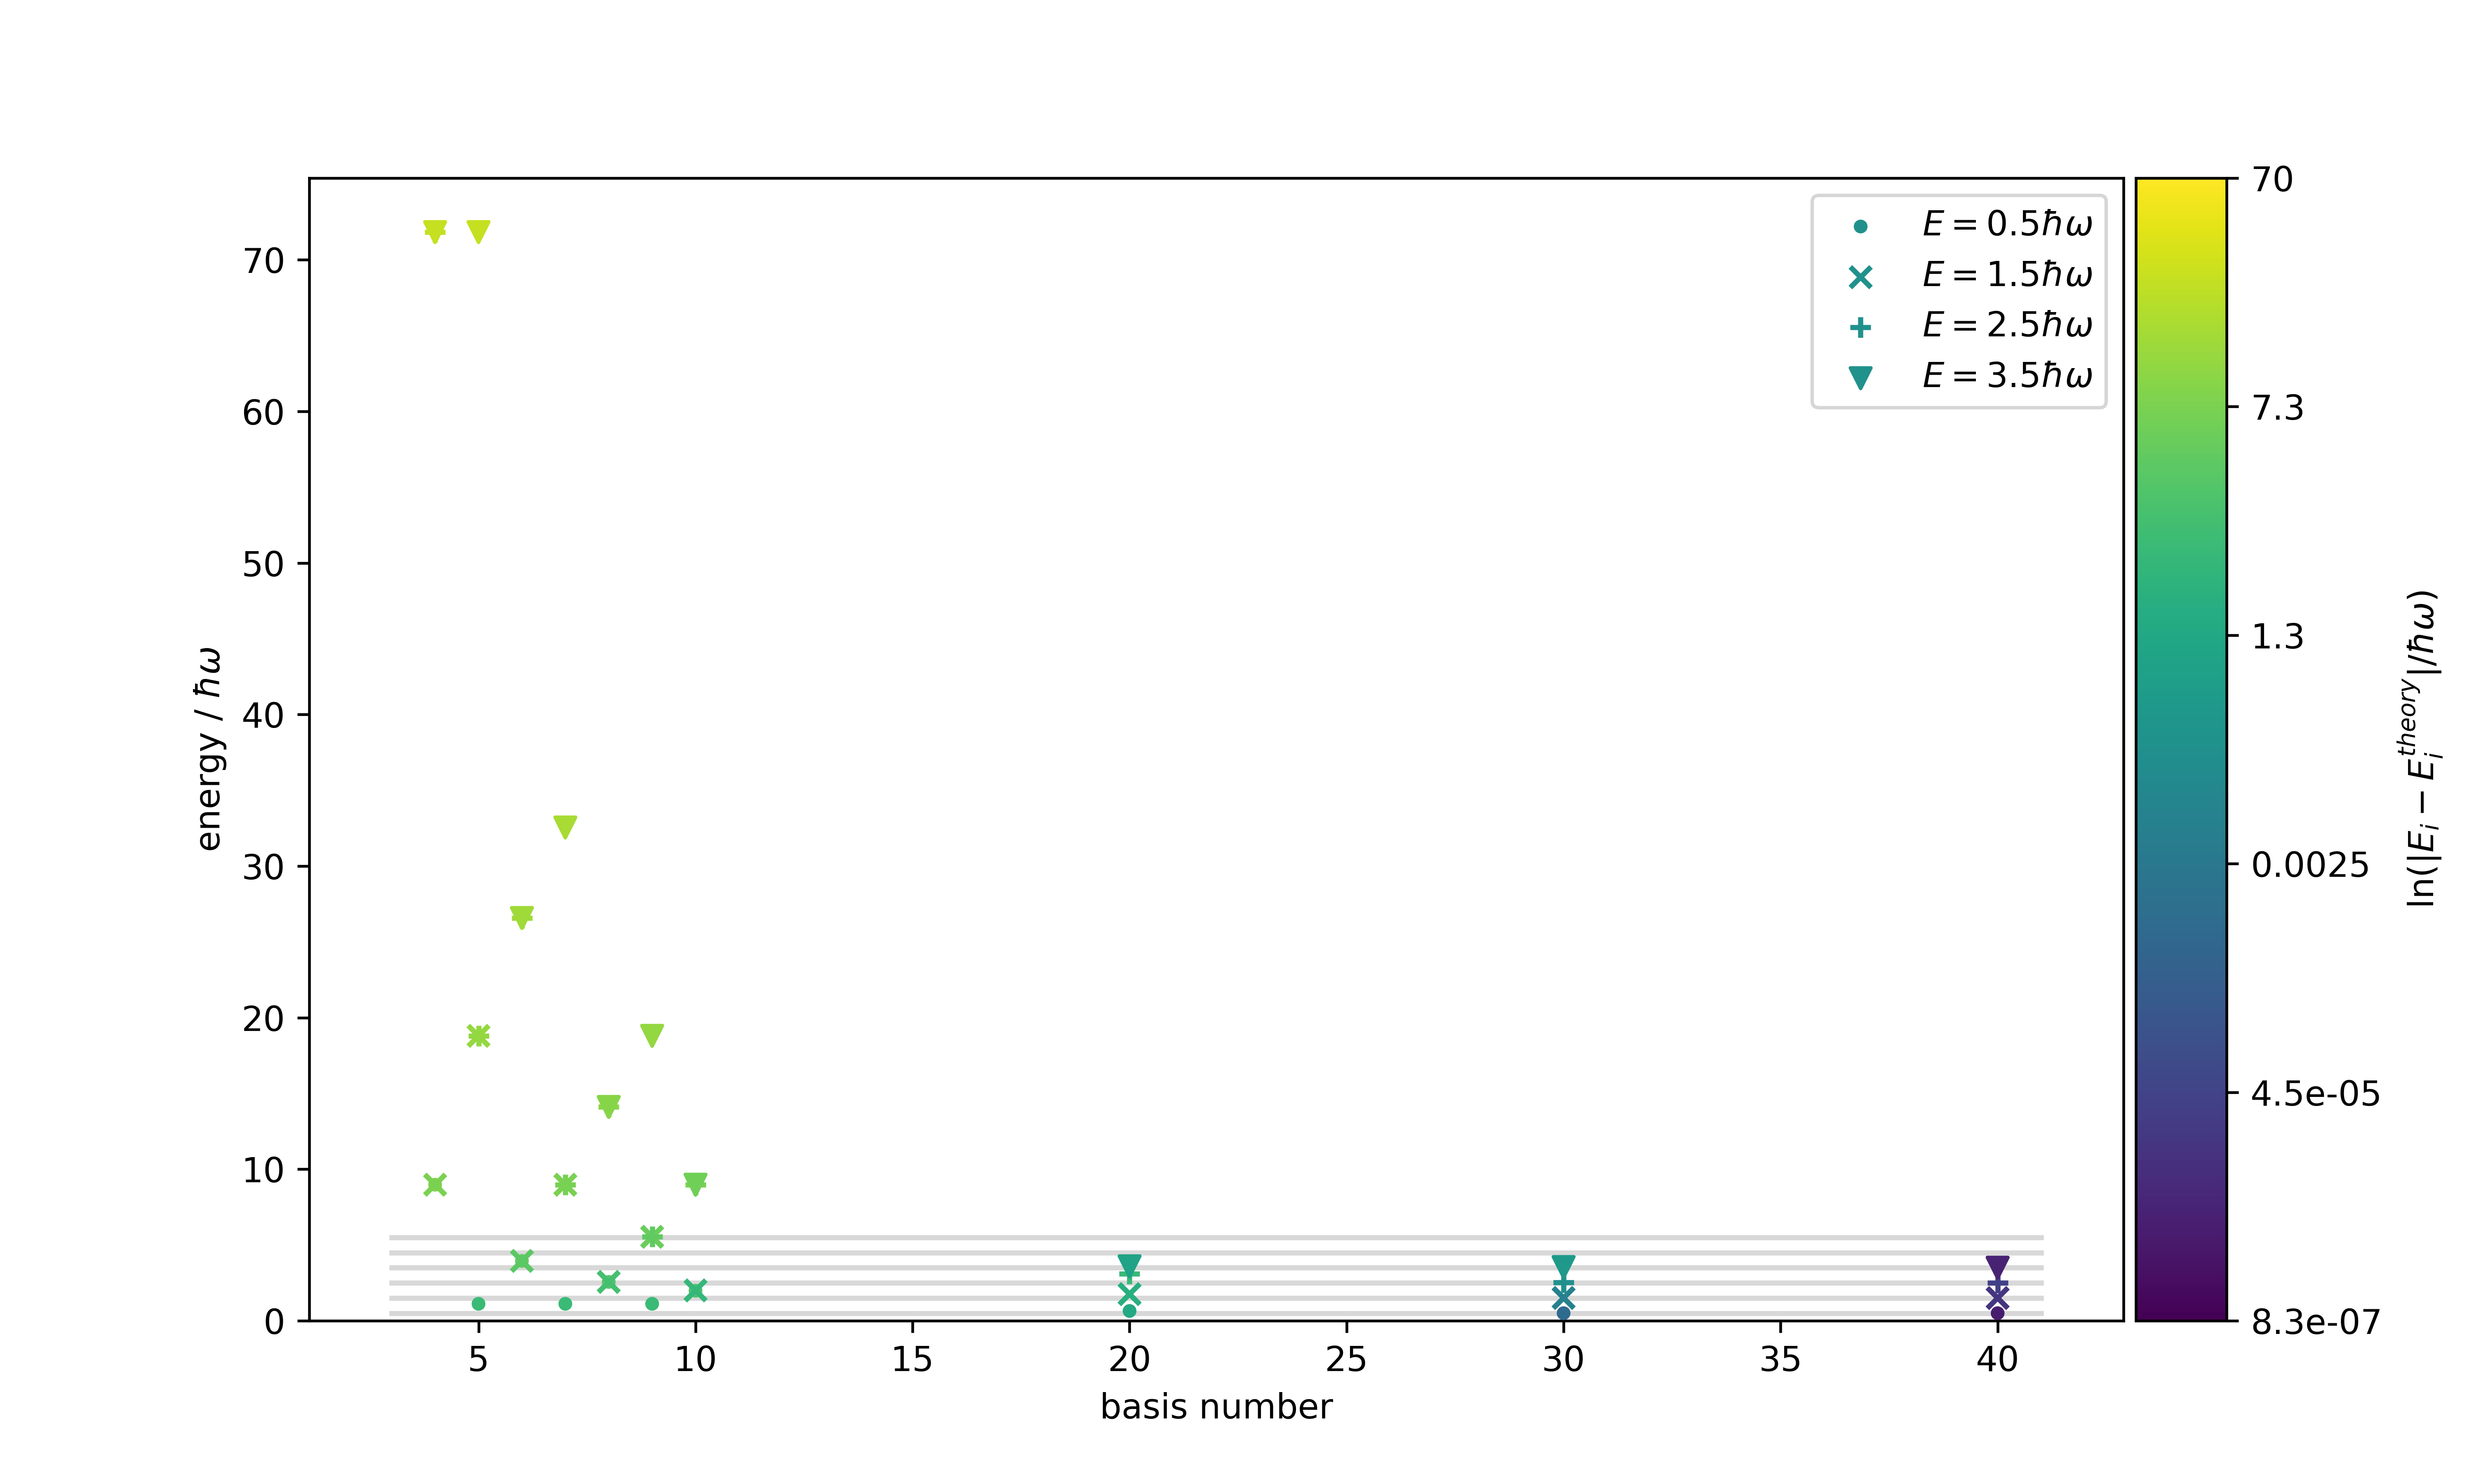
\includegraphics[width=1\textwidth]{V_1_Center_different basis number.png}
    \caption{Many basis required to get precise result with varying center basis. The color characterizes how close the numerical result is to the theoretical value.}
    \label{fig:V1_dif_basis_num_center}
\end{figure}

\begin{figure}[!htb]
    \centering
    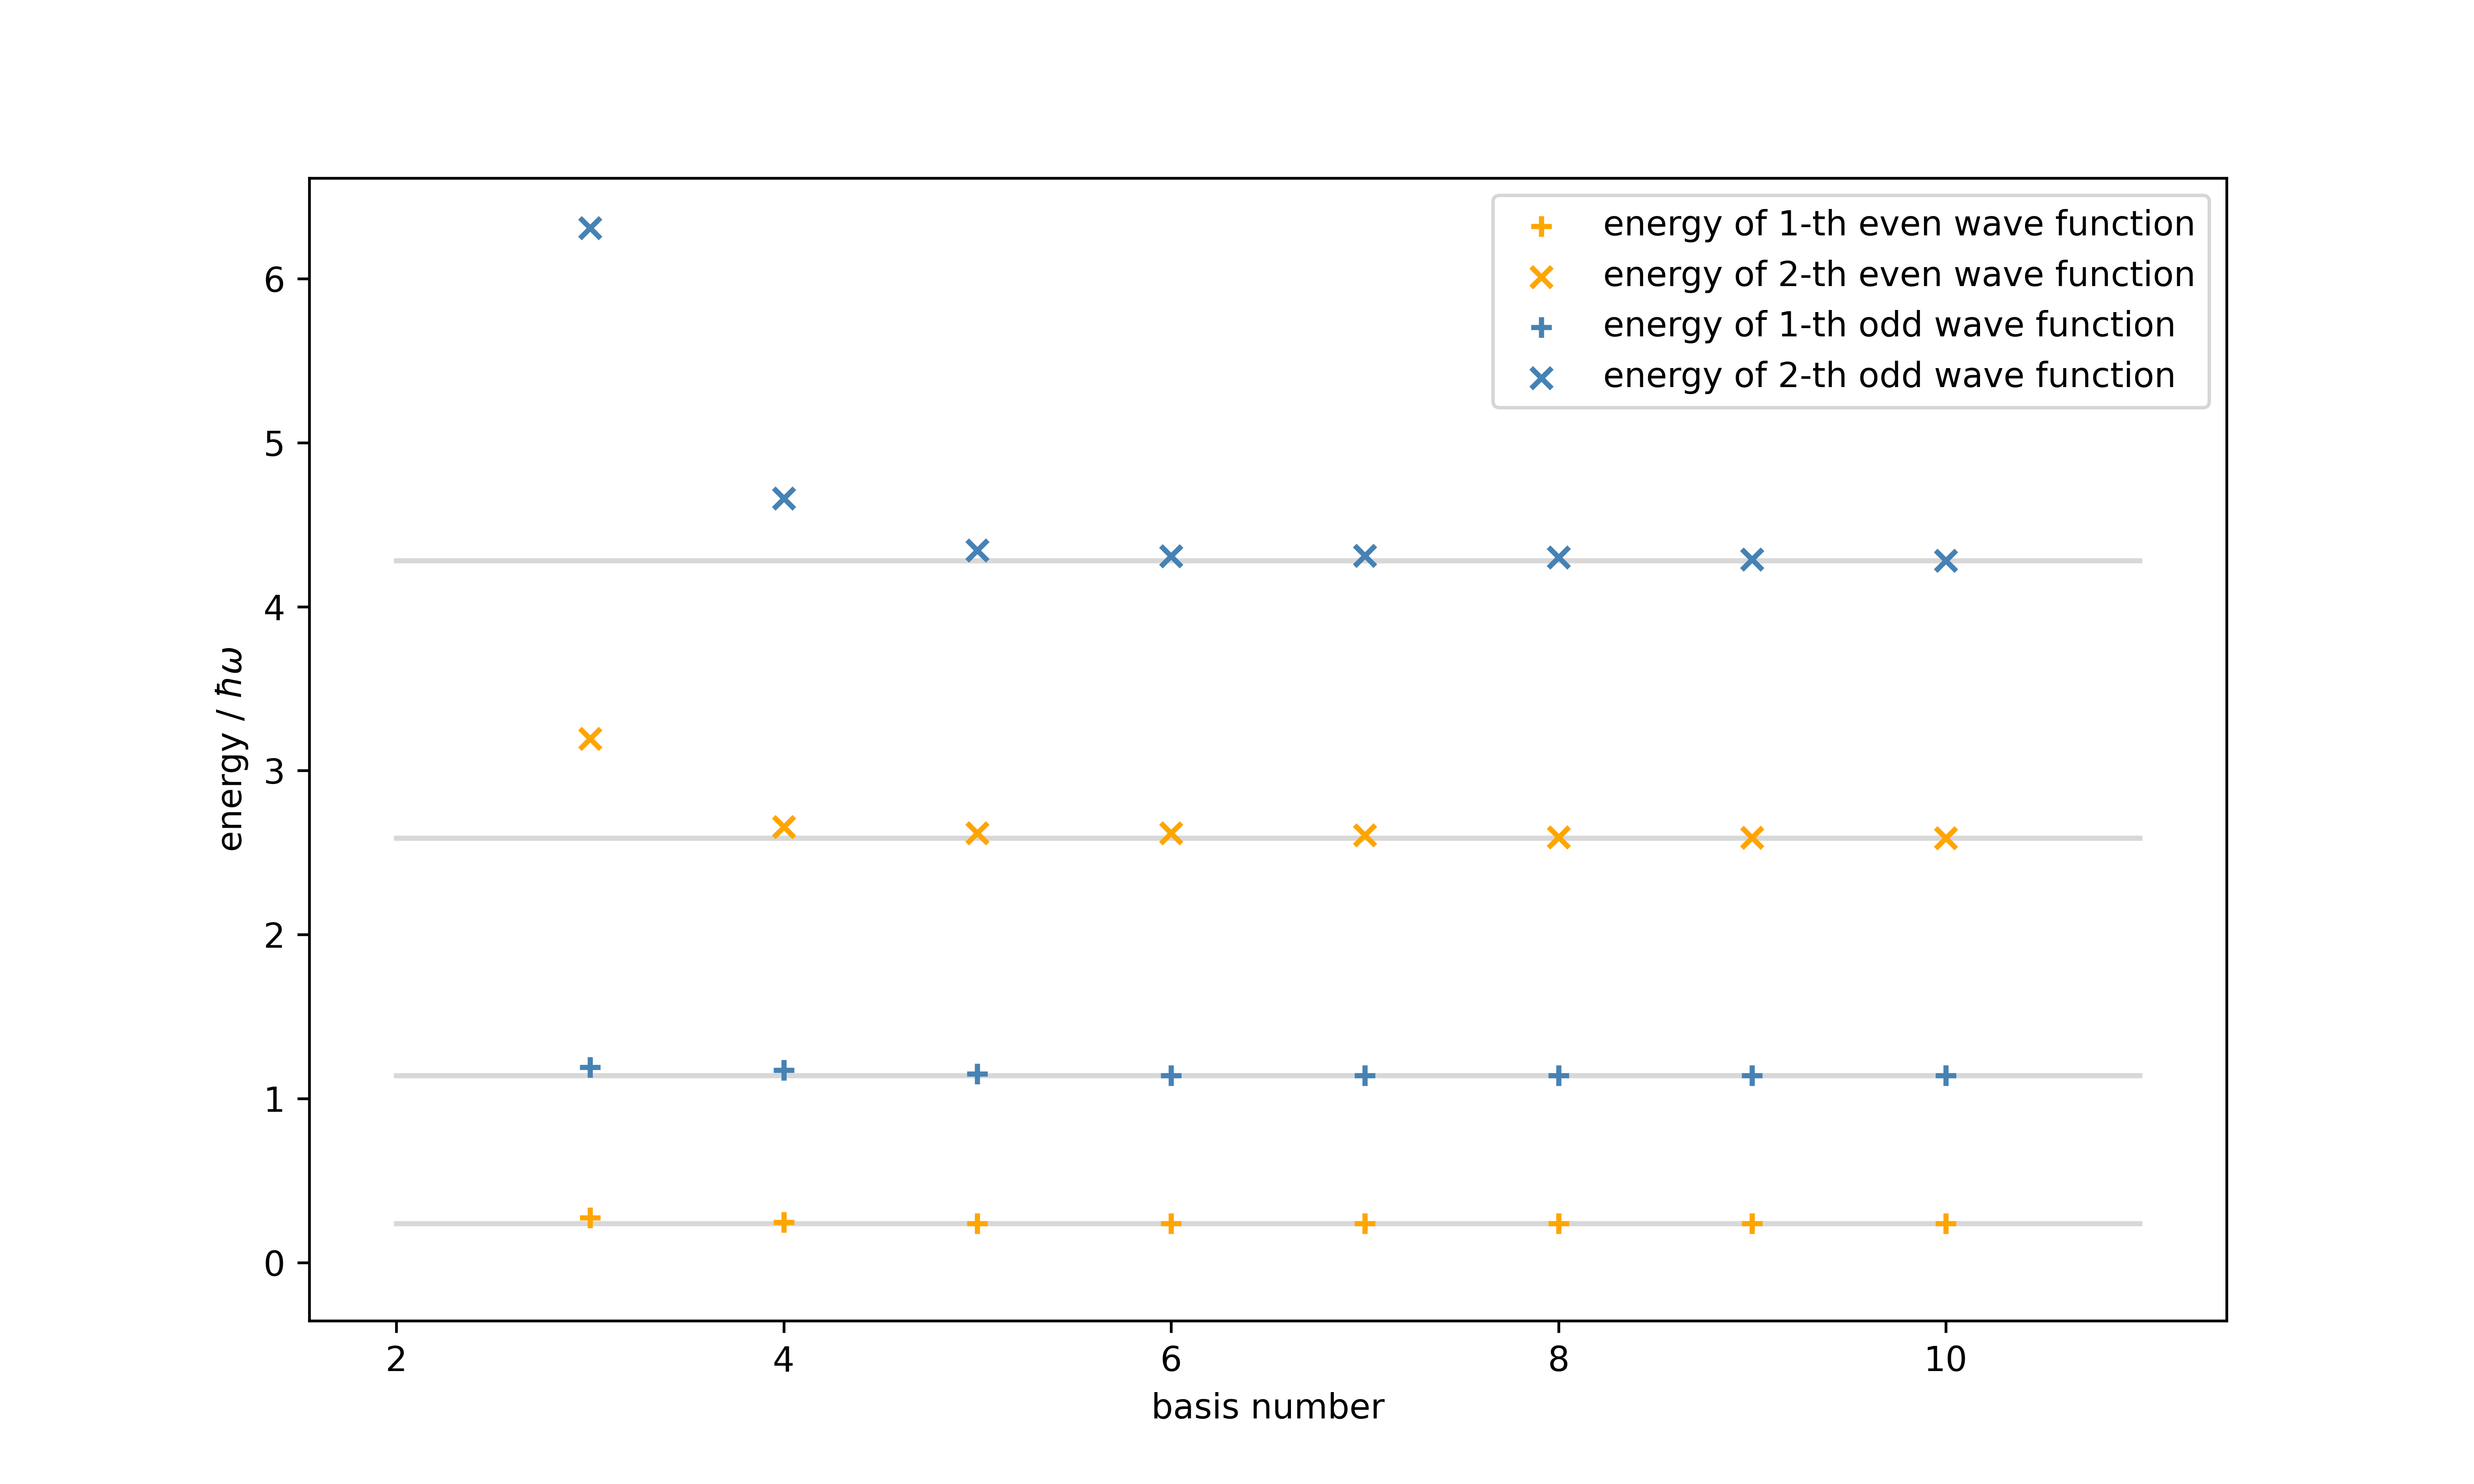
\includegraphics[width=1\textwidth]{V2even_and_odd_different_basis.png}
    \caption{Many basis required to get precise result with varying center basis.}
    \label{fig:V2_dif_basis_num_center}
\end{figure}

\begin{figure}[!htb]
    \centering
    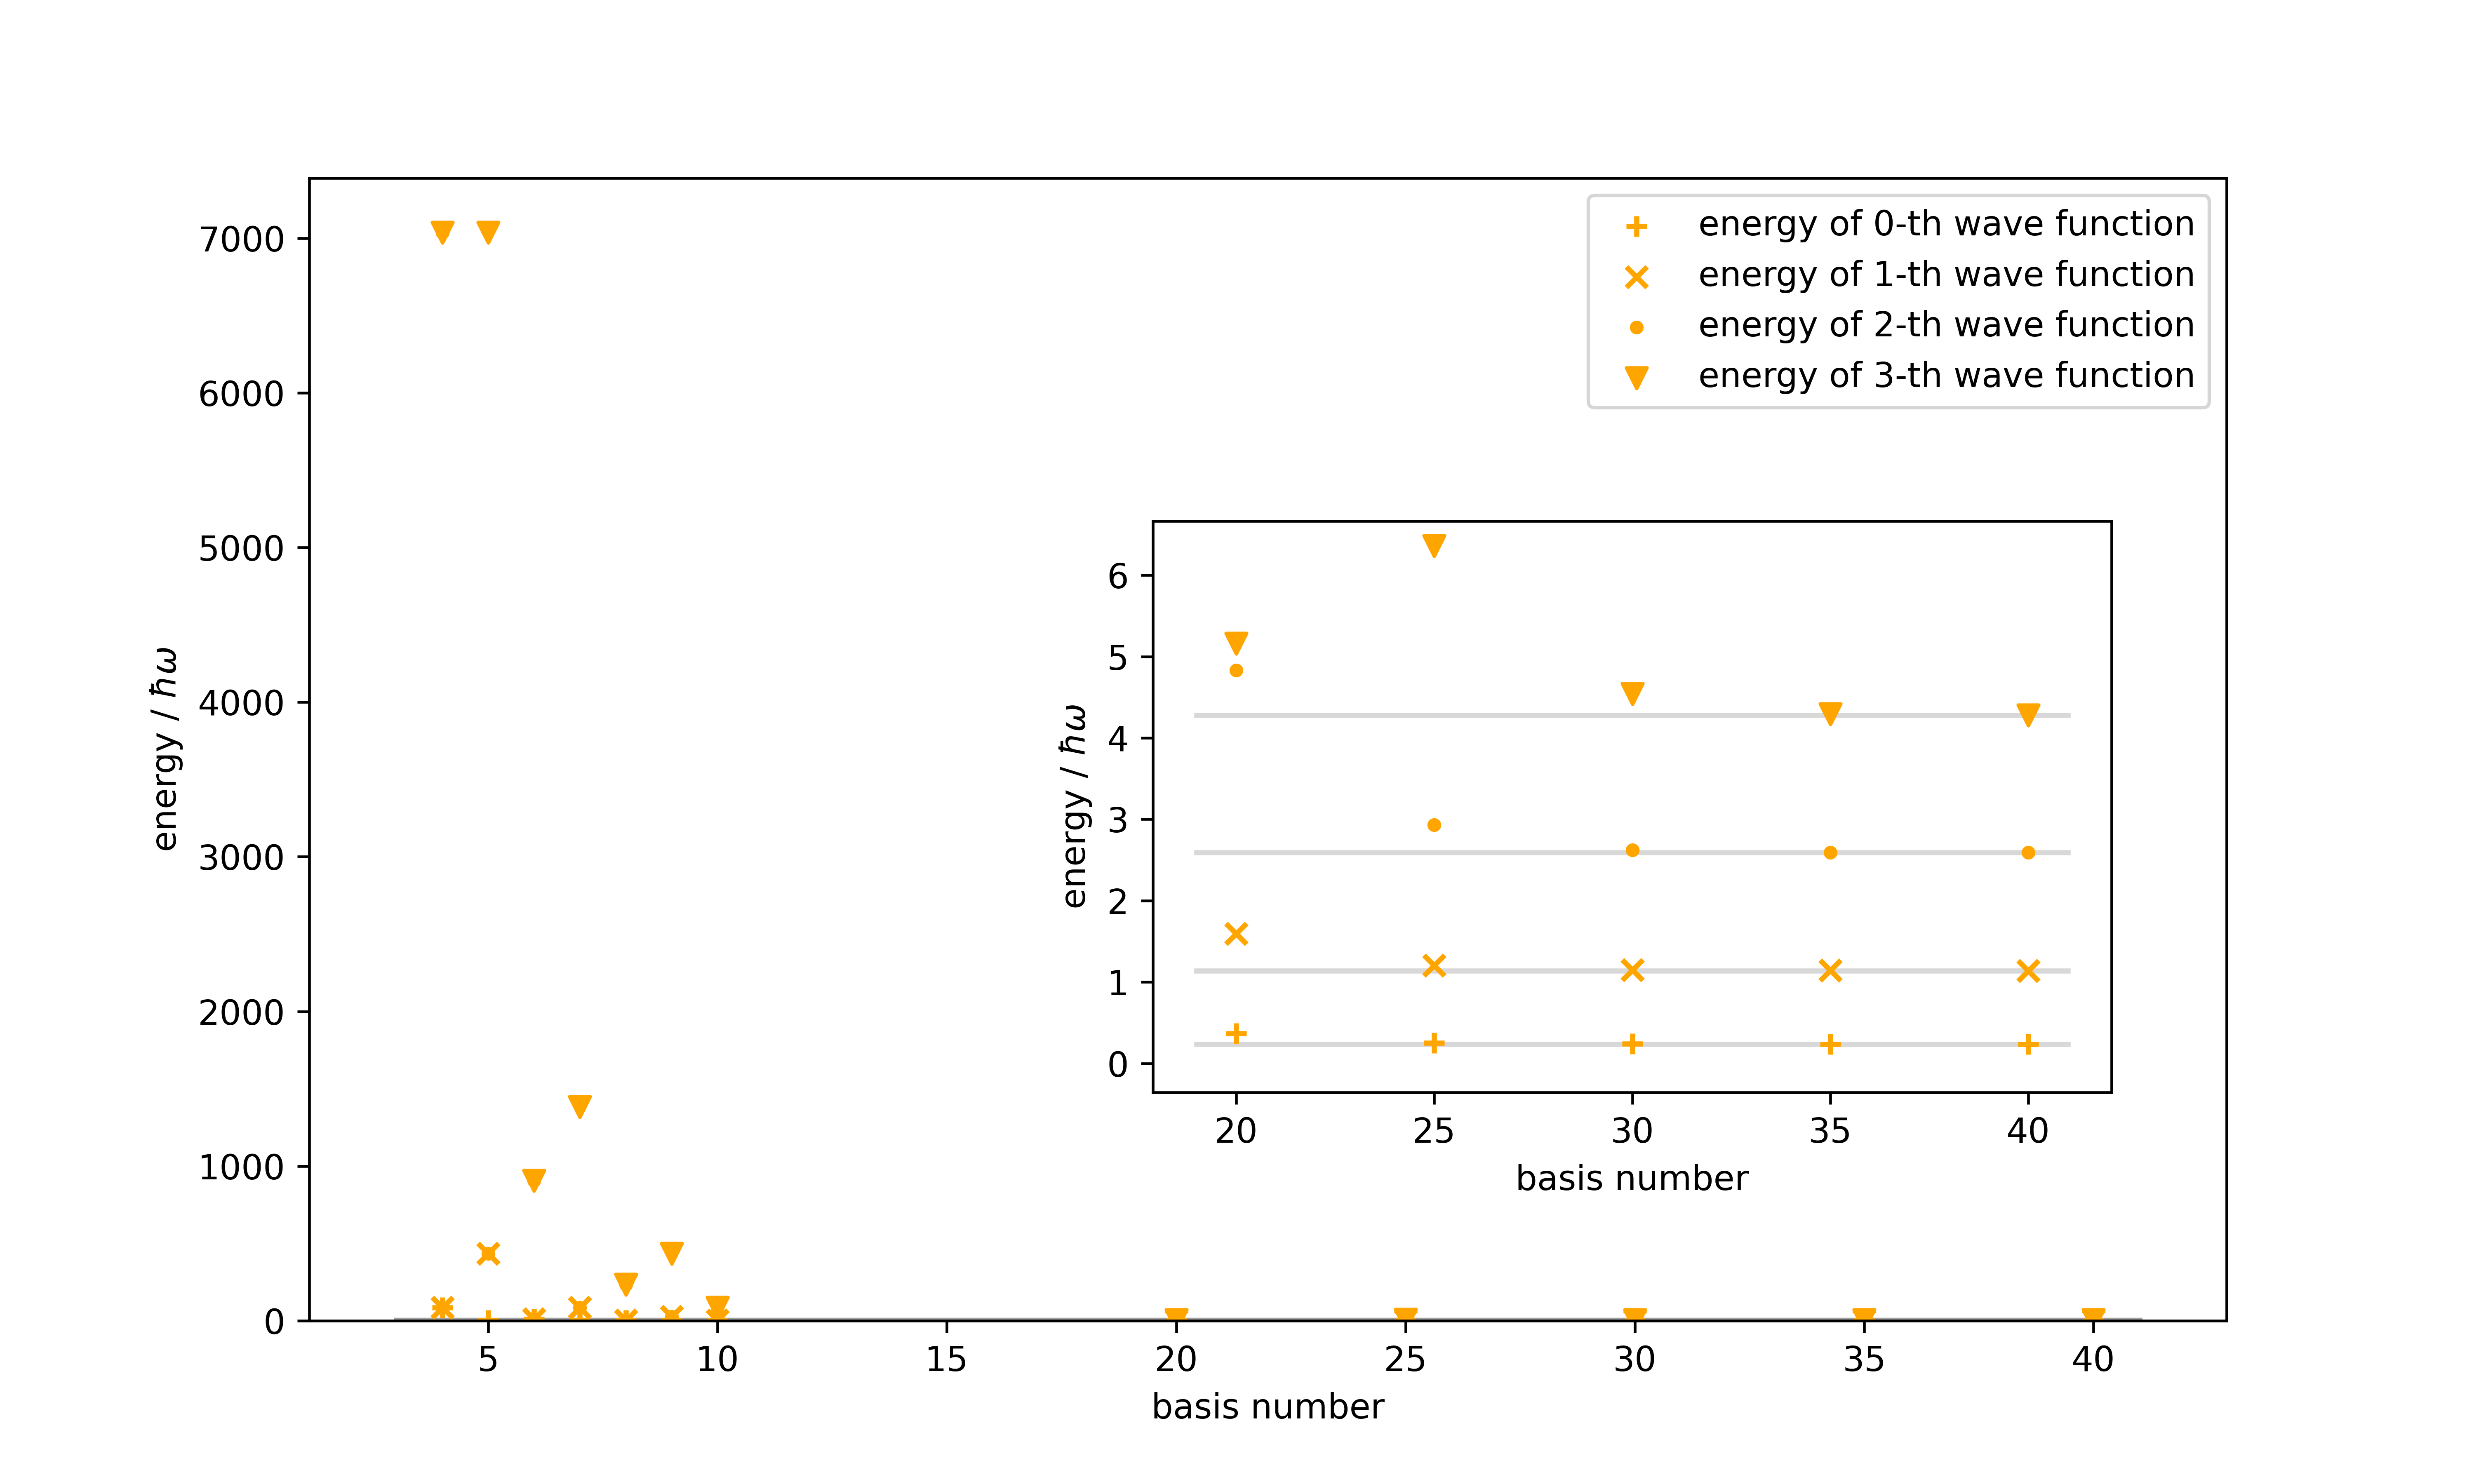
\includegraphics[width=1\textwidth]{V2_center_differen_basis.png}
    \caption{Few basis is required for 'varying width Gaussian and Eq.\ref{basis_odd_and_even}' basis to give accurate results}
    \label{fig:V2_dif_basis_num_even_and_odd}
\end{figure}

\end{document}




